\chapter{{A proposed workflow}}\label{workflow}

After the analysis of existing subtitling guidelines, their shortcomings, the \isi{graphical translation} of text elements, and the summary of common \isi{placement} strategies, the impression hardened that strict norms or guidelines for integrated titles would not be the right solution for such an individual and artistic medium like film.\footnote{Parts of this chapter are also published in the book chapter “A proposed workflow for the creation of integrated titles based on \isi{eye tracking} data” in the book “Seeing into screens: Eye tracking and the moving image” (2017, Bloomsbury).} The many possibilities to work creatively with text elements, \isi{typography}, and \isi{image composition} as well as extensive discussions with filmmakers and subtitle professionals also played an important part in this decision. Therefore, a concept for modular guidelines and recommendations for the creation of integrated titles was created that could be combined based on individual requirements. The following steps were identified as essential for the workflow:

\begin{itemize}
\item Translation process
\item Analysis
\item Operationalisation
\item Application
\end{itemize}

The \isi{translation process} includes the first draft as well as corrections and adjustments throughout the whole process. However, the major part of the \isi{translation process} should be complete before starting with the other steps – the analysis of the film material, decision on strategies that will be used, and the application of both. These steps are illustrated in the following chart (\figref{fig:FIG43}).

\begin{figure}
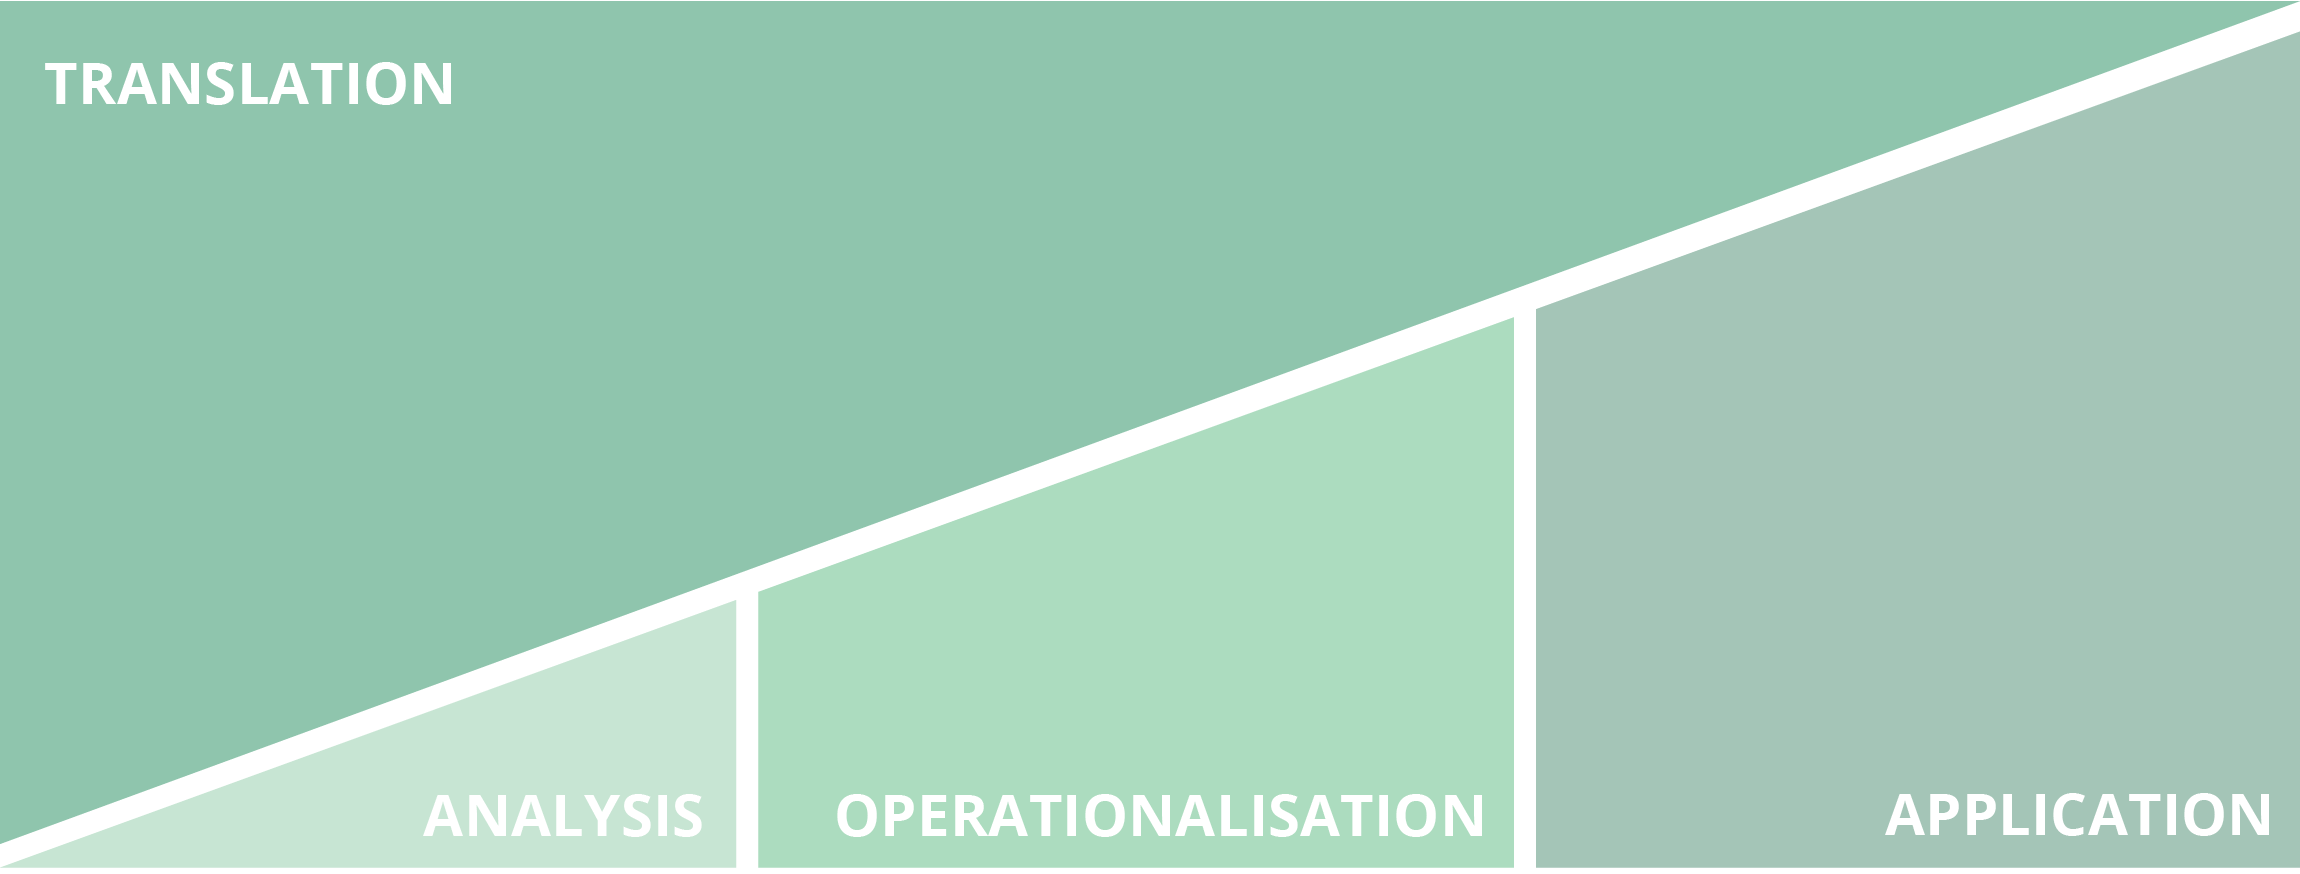
\includegraphics[width=\textwidth]{figures/FIG43chart1.png}
\caption{Relevant steps for the creation of integrated titles}
\label{fig:FIG43}
\end{figure}

Except for the \isi{translation process} that is described and discussed in detail in many other places as well as in \sectref{sec:1.2.2}, the other three modules and the connected tasks are presented in the following sections.

\section{Analysis}\label{sec:5.1}

The analysis of the film material should include the \isi{image composition} and the filmmaker’s intentions (see \sectref{sec:3.3}), a definition of the overall complexity of the film and individual scenes (as this influences the use of \isi{placement} strategies, effects, and \isi{layout}), and an understanding of the \isi{typographic identity} of the film. Additionally, a look at the target group is important.



The question whether the target group is made up of a hearing or a \isi{deaf audience} and whether it uses a spoken language or sign language as first language can easily influence \isi{placement} and \isi{layout} strategies. The following possible purposes of subtitles should be taken into account:


\begin{itemize}
\item Interlingual translation
\item Intralingual translation
\item Intralingual translation for the prelingually \isi{deaf}
\item Intralingual translation for the postlingually \isi{deaf} and hard-of-hearing
\end{itemize}

Especially the differenciation between a hearing and a hard-of-hearing or \isi{deaf audience} as well as the differences within the hearing-impaired group should be taken into account – this includes the difference between being born \isi{deaf} or having become \isi{deaf} postlingually:
\begin{quote}
People who are born hearing and become \isi{deaf} late in life, are “physically \isi{deaf}”, but “culturally hearing”. They grew up speaking a spoken language, using the telephone, the TV, the radio. They think, speak, read, write and base their opinions on the world they knew before they became \isi{deaf}. They rarely learn a signed language. People who are born into the Deaf Community, and whose first native language is a signed language, not a spoken one, are “culturally Deaf”. Most of them are physically \isi{deaf} as well. Some of them are born \isi{deaf} or became \isi{deaf} at a very young age. Some of them are hearing people born into all-\isi{deaf} families, and even though they can hear, even though they speak a spoken language, their first language was a signed language, not a spoken language. They base their view of the world from the Deaf perspective. They are “physically hearing” but “culturally-\isi{deaf}”. (\citealt{sutten????})
\end{quote}
It can be assumed that hearing-impaired audiences are more interested in additional \isi{layout} effects such as the colour-based indication of speakers. Furthermore, it is likely for prelingually \isi{deaf} audiences to demonstrate a lower reading pace (\citealt{Dyer2003}:~215ff.).\footnote{Cf. \url{https://www.valdosta.edu/student/disability/documents/captioning-key.pdf} [2016--08--12].}

Together with the translation, an analysis of content and situations should take place. The pace of speech acts, music and sound, and the existence, number, and \isi{layout} of text elements can influence the space and time available for the integrated titles. As these aspects are tightly connected to the image and as discussed in \sectref{sec:3.3} on the influence of film studies on the creation of integrated titles, a basic understanding of \isi{image composition} rules should be present. Aspects of filmmaking such as angles, lenses, depth perception, cuts, etc. help to understand how a shot works, what format it is, and what content is presented in what way. Only if the \isi{image composition} and image systems that are at work are understood, can primary and secondary areas be defined and a good position for a title be found. As concluded in \sectref{sec:3.5}, a basic understanding of the following aspects as well as of film studies and the filmmaker’s intentions should help to interpret atmosphere and tone:

\begin{itemize}
\item Shot compositions
\item Tools and rules
\item Emotion + Story (e.g. for \isi{layout}, but also timing and content translation)
\item Rhythm (e.g. for title timing)
\item Eye-trace (title \isi{placement})
\item Use of three-dimensional space (\isi{speaker identification}, \isi{indication of speaking direction}, atmosphere)
\item Image systems (titles should follow a continuative system that provides \isi{recognition value} and supports the film without becoming the \isi{main focus})
\end{itemize}

Being a combination of these and further aspects mentioned in \sectref{sec:3.3}, films and individual scenes can be assigned various levels of difficulty concerning the \isi{placement} of integrated titles. These levels of difficulty are based on a number of characteristics that can either complicate the title \isi{placement} or make it easier:


\begin{itemize}
\item \textit{Static scenes (easier) vs. more active scenes (harder)}: In a static scene with little movement (concerning both camera and elements in the image), the title \isi{placement} is almost as easy as when designing a poster.\footnote{Cf. \url{http://www.pro-media.org/download/VISATT-Analyse.pdf} [2016--08--12] on effective \isi{text placement} in poster design.} It is less likely for the background – and therefore, the contrast – of a title to change abruptly or an important element to move behind the title. With increasing movement in the scene or of the camera, \isi{placement} becomes more difficult.
\item \textit{No visible speaker vs. one or more visible speakers}: As faces and \isi{gaze} directions are salient features and strong eye catchers, a larger number of visible persons – especially speakers – increases the difficulty of title \isi{placement}. Speakers are a \isi{primary area} of the image that should not be covered by a title – at least not the face or other parts of the body that are obviously the \isi{main focus} in the scene. With a single visible speaker, there’s usually enough secondary space for title \isi{placement} and movement can still be integrated or at least balanced. With an increasing number of visible speakers, less and less secondary image area is left for the titles. Close-ups, especially of the face, pose an additional challenge.
\item \textit{Speaker inside the frame vs. speaker outside the frame}: This characteristic is comparable to the number of visible speakers. However, with a speaker outside the frame, it is still possible to indicate his or her position in relation to the frame.
\item \textit{No cuts during speech act vs. cuts during speech act}: Cuts change the image and, if taking place during speech, can cause the area behind a title to cease providing \isi{sufficient contrast}, or might even contain a relevant element that should not be covered.
\item \textit{Secondary area is predominant vs. \isi{primary area} is predominant}: The \isi{primary area} usually includes speakers’ faces, elements that are in the \isi{main focus} due to the lense and editing, as well as elements the speaker relates to by looking at, mentioning, touching it, etc. (see \sectref{sec:7.5.2}). The remaining area can usually be defined as secondary and be covered by titles.
\item \textit{Strong contrast vs. weak contrast}: This characteristic is mostly self-explan\-a\-to\-ry. An even image can provide a strong contrast and therefore ease title \isi{placement} while a chaotic or very bright image can make it difficult. The \isi{layout} of the titles can be adjusted by using a strong outline or shadow.
\end{itemize}

The translation and the analysis of the image are closely linked and together make up the content analysis. The complexity and form of both are determined for the film and individual scenes: Do monologues outweigh dialogues, are there many quick-paced fights or rather formal greetings and discussions, where are the speakers in relation to other focus points, and are there many pre-existing text elements in the image? These considerations allow for first basic decisions concerning \isi{placement} and \isi{layout} strategies. The \isi{layout} strategies are not only based on the content and complexity, however, but should also be preceded by an analysis of the \isi{typographic identity} of the film. Type faces, colours, and existing \isi{placement} and effect strategies should be considered and incorporated in the \isi{layout} of the integrated titles (see \sectref{sec:2.3}).

\section{Operationalisation}\label{sec:5.2}

Based on the criteria developed in \chapref{overview} and \chapref{integrated}, the following characteristics are required from integrated titles:

\largerpage
\sloppy
\begin{itemize}
\item Intuitiveness (\isi{learnability}, efficiency, and \isi{memorability})
\item Usefulness


\begin{itemize}
\item Suitable translation (e.g. preventing \isi{negative acoustic feedback} effects)
\item Consistency (following comprehensible rules and avoid irritation, frustration or amusement when not intended)
\item Readability / \isi{legibility}
\item Reduced \isi{eyestrain} (small distance in between consecutive titles)
\item Close to action and close to speaker (\isi{speaker identification})
\end{itemize}
\item Satisfaction, based on the combination of pleasant \isi{layout} and \isi{comprehensible design concept}:


\begin{itemize}
\item Titles are within \isi{safe area}
\item Suitable \isi{typeface}
\item Legible colour combinations
\item Saturation index <85\,\%
\item Not obscuring speaker’s mouth, other text elements or important activity
\end{itemize}
\end{itemize}
\fussy

Provided with full access to existing text elements and this basic set of additional skills, the creation of integrated titles should be possible. However, especially the sources on \isi{usability} demand comprehensible rule sets for titles (at least within a film). \chapref{placement} therefore analysed the \isi{placement} strategies of commercial integrated titles and provided the basic positions as listed in \tabref{tab:TAB13}.

\begin{table}
\begin{tabularx}{\textwidth}{XX}
\lsptoprule
 Visible speakers &  Placement strategy\\
 \midrule 
 Off-screen & Below focus\\
& Next to focus\\
& Speaking direction\\
\tablevspace
 1 Speaker & Below speaker\\
& Next to speaker\\
& Speaking direction\\
\tablevspace
 2+ Speakers & Below focus / speaker\\
& Next to focus / speaker\\
& In between speakers\\
\lspbottomrule
\end{tabularx}
\caption{Basic set of positions for integrated titles developed in \chapref{placement}}
\label{tab:TAB13}
\end{table}

These positions can of course be combined with more individual positions based on the film’s \isi{image composition} and atmosphere. While these positions describe the actual physical position in relation to the speaker, it should be based on a specific concept, ideally developed for each film individually. Based on the so far mentioned criteria, a number of \isi{layout} and \isi{placement} objectives can be derived. The following list constitutes a first draft and can be expanded as needed:

\sloppy
\begin{itemize}
\item \textit{Short distances for high(er) information processing}: As the eye movements between focus points are so fast that no information can be absorbed or processed (see \sectref{sec:6.1}), one objective can be to place titles as close as possible to \isi{main focus} areas to decrease loss of information. For the present study, these \isi{main focus} areas could be clearly defined based on the recorded eye movements. With integrated titles being closer to the \isi{main focus} areas, the viewing behaviour of audiences watching a film with integrated titles is more likely to resemble the natural viewing behaviour of an audience that does not require a translation. This objective can therefore also be called \textsc{natural focus}.
\item \textit{No coverage of primary areas}: If the \isi{image composition} is to be taken especially into account and no primary areas or elements should be covered, \isi{eye tracking} data could be used here as well to define these areas. Basic knowledge of film studies and \isi{communication design} principles (see \sectref{sec:3.1} and \sectref{sec:3.3}) can also help with the analysis and interpretation of film scenes.
\item \textit{Indication of speaker and speaking direction}: The position of a title can take place in a way that makes it possible to connect the title quickly to the speaker (e.g. below a speaker). Furthermore, the position of a title can also indicate \isi{speech direction} or the position of the conversation partner. This also supports a \isi{natural focus}, e.g. in a conversation between two speakers with the titles placed in between them.
\item \textit{Legibility}: Good \isi{legibility} and \isi{readability} are usually achieved through a strong contrast and even background. A well-designed title can still be read in front of a changing background and reflects the image’s \isi{colour concept} rather than disturbing it (while still creating a strong enough contrast to be read easily).
\item \textit{Individual \isi{aesthetic} and/or \isi{typographic} concepts}: Other concepts might focus less on \isi{usability} but rather on supporting a film’s atmosphere, tone, or \isi{image composition}. This can be reflected by the \isi{typographic identity}, effects, or special \isi{placement} strategies (cf. \textit{John Wick}).
\item \textit{Accessibility}: Finally, accessibility can be the reason for the use of integrated titles in a film. This might include already mentioned objectives such as the \isi{speech direction} indication but also additional ones such as \isi{noise indication} or \isi{colour-based speaker identification}.
\end{itemize}
\fussy

When deciding what objectives should be reached through the concept for the integrated titles for a specific film, it should be clear from the beginning whether the overall concept is primarily artistic (see e.g. \textit{Man on Fire} and \textit{Slumdog Millionaire}) or the aim is to improve the overall \isi{legibility} and \isi{information intake} (as was the purpose of the present study). Additionally, concepts can include aims such as transportation or immersion that have been shown to even increase through the existence of subtitles or titles in a film.\footnote{Cf. “The Impact of Subtitles on Psychological Immersion”, Prof.~Dr.~Jan-Louis Kruger, Macquarie University, Australia, and Vaal Triangle Campus, North-West University, South Africa, “Languages \& The Media” conference in Berlin [2014--11--06].\\
}

Another topic that should be taken into consideration is effects. While this has not been studied in the present experiment or the analysed films in the previous chapters, they definitely play a relevant role and present an interesting topic for a follow-up study. The following effects were present in the films with integrated titles analysed in \chapref{placement}:

\sloppy
\begin{itemize}
\item \textit{Kinetic effects}: These are titles that illustrate motion, e.g. by moving over the screen or being placed consecutively in a way that indicates motion (cf. \textit{Heroes}). Moving titles were visible multiple times e.g. in \textit{Man on Fire} moving in and out of the frame or in \textit{Nochnoy Dozor} following an object that is thrown towards a person.
\item \textit{Spatial effects}: Some titles are edited in a way that it seems like another element in the image is in front of it, e.g. a person walking by will cover the title when passing. This was done in \textit{Man on Fire}, \textit{John Wick}, \textit{Nochnoy Dozor}, and \textit{Fast Five}.
\item \textit{Repetitive effects}: Some titles were repeated additionally, e.g. before and after cuts or to emphasize a statement (\textit{Man on Fire}, \textit{Nochnoy Dozor}).
\item \textit{Transformative effects}: These effects cover a wide range of possibilities that seems unlimited due to today’s tools and software. For example, \textit{Man on Fire} has titles that disperse and leave focus because the speaker is crying and \textit{Nochnoy Dozor} features titles that disperse into a blood trail to illustrate the speaker being a vampire on the hunt.
\item \textit{Display effects}: While conventional subtitles are usually displayed uniformly, this can also be adjusted. Titles can be faded in and out faster or slower to indicate speech pace or emotions, they can be displayed letter by letter or line by line, they can blur in or out, etc. (see \textit{Man on Fire}).
\item \textit{Typographic effects}: The \isi{layout} and especially \isi{typography} of a title can also convey information – \isi{font} size or form (e.g. capitals) can visualise volume, specific fonts can cause certain associations, etc.
\end{itemize}
\fussy

For the present study, the following effects were used, aiming to support the atmosphere and increase the information flow:

\begin{itemize}
\item \textit{Fade in/out}: Slow, emotional or hesitant statements are faded in and out slowly. Sentences that are left unfinished are faded out slowly, while quick and clear or confident speech kept with the usual quick fade in and out.\footnote{The film encyclopedia of the University of Vienna offers some definitions and examples on fading effects, see \url{https://wiki.univie.ac.at/pages/viewpage.action?pageId=35751449} [2016--08--15].}
\item \textit{Simultaneity}: Displayed at the same time, integrated titles can indicate multiple speakers talking simultaneously.
\item \textit{Depth effect}: Several titles simulate depth as titles are briefly covered by a speaker’s hand as he or she makes big gestures, or when someone moves a little bit in front of a title. Before a title was covered, it was made sure that it was completely visible long enough to be read properly. 
\end{itemize}

Depending on the individual film, genre, and intentions, a wide range of effects is possible and can be used to support the film’s atmosphere but also increase the \isi{entertainment value} and maybe even the accessibility of the film.

\section{Application}\label{sec:5.3}

After a decision has been made on the strategies as well as the \isi{layout} for the titles, it’s time to place the integrated titles in the film – using the chosen \isi{layout}. In order to do this, the first step should be to identify the focus points in the scene based on the analysis of the film and its \isi{image composition}. This can be achieved by dividing the image visible during a speech act (or music or noise, etc.) into primary and secondary areas. The integrated titles should then be placed in the secondary areas where possible and not cover primary areas and elements. Next, the chosen \isi{layout} features should be controlled – do the titles look the way planned and have the intended effect? Also, the contrast should always be strong enough to ensure \isi{legibility} (unless illegibility is intended). During a final check, the need for additional information or additional effects should be analysed. Additional information might be necessary for fully accessible titles, and additional effects might be required in order to support a film’s specific tone and atmosphere.

\figref{fig:FIG44} gives a final overview over the proposed workflow for the creation of integrated titles.

\begin{figure}
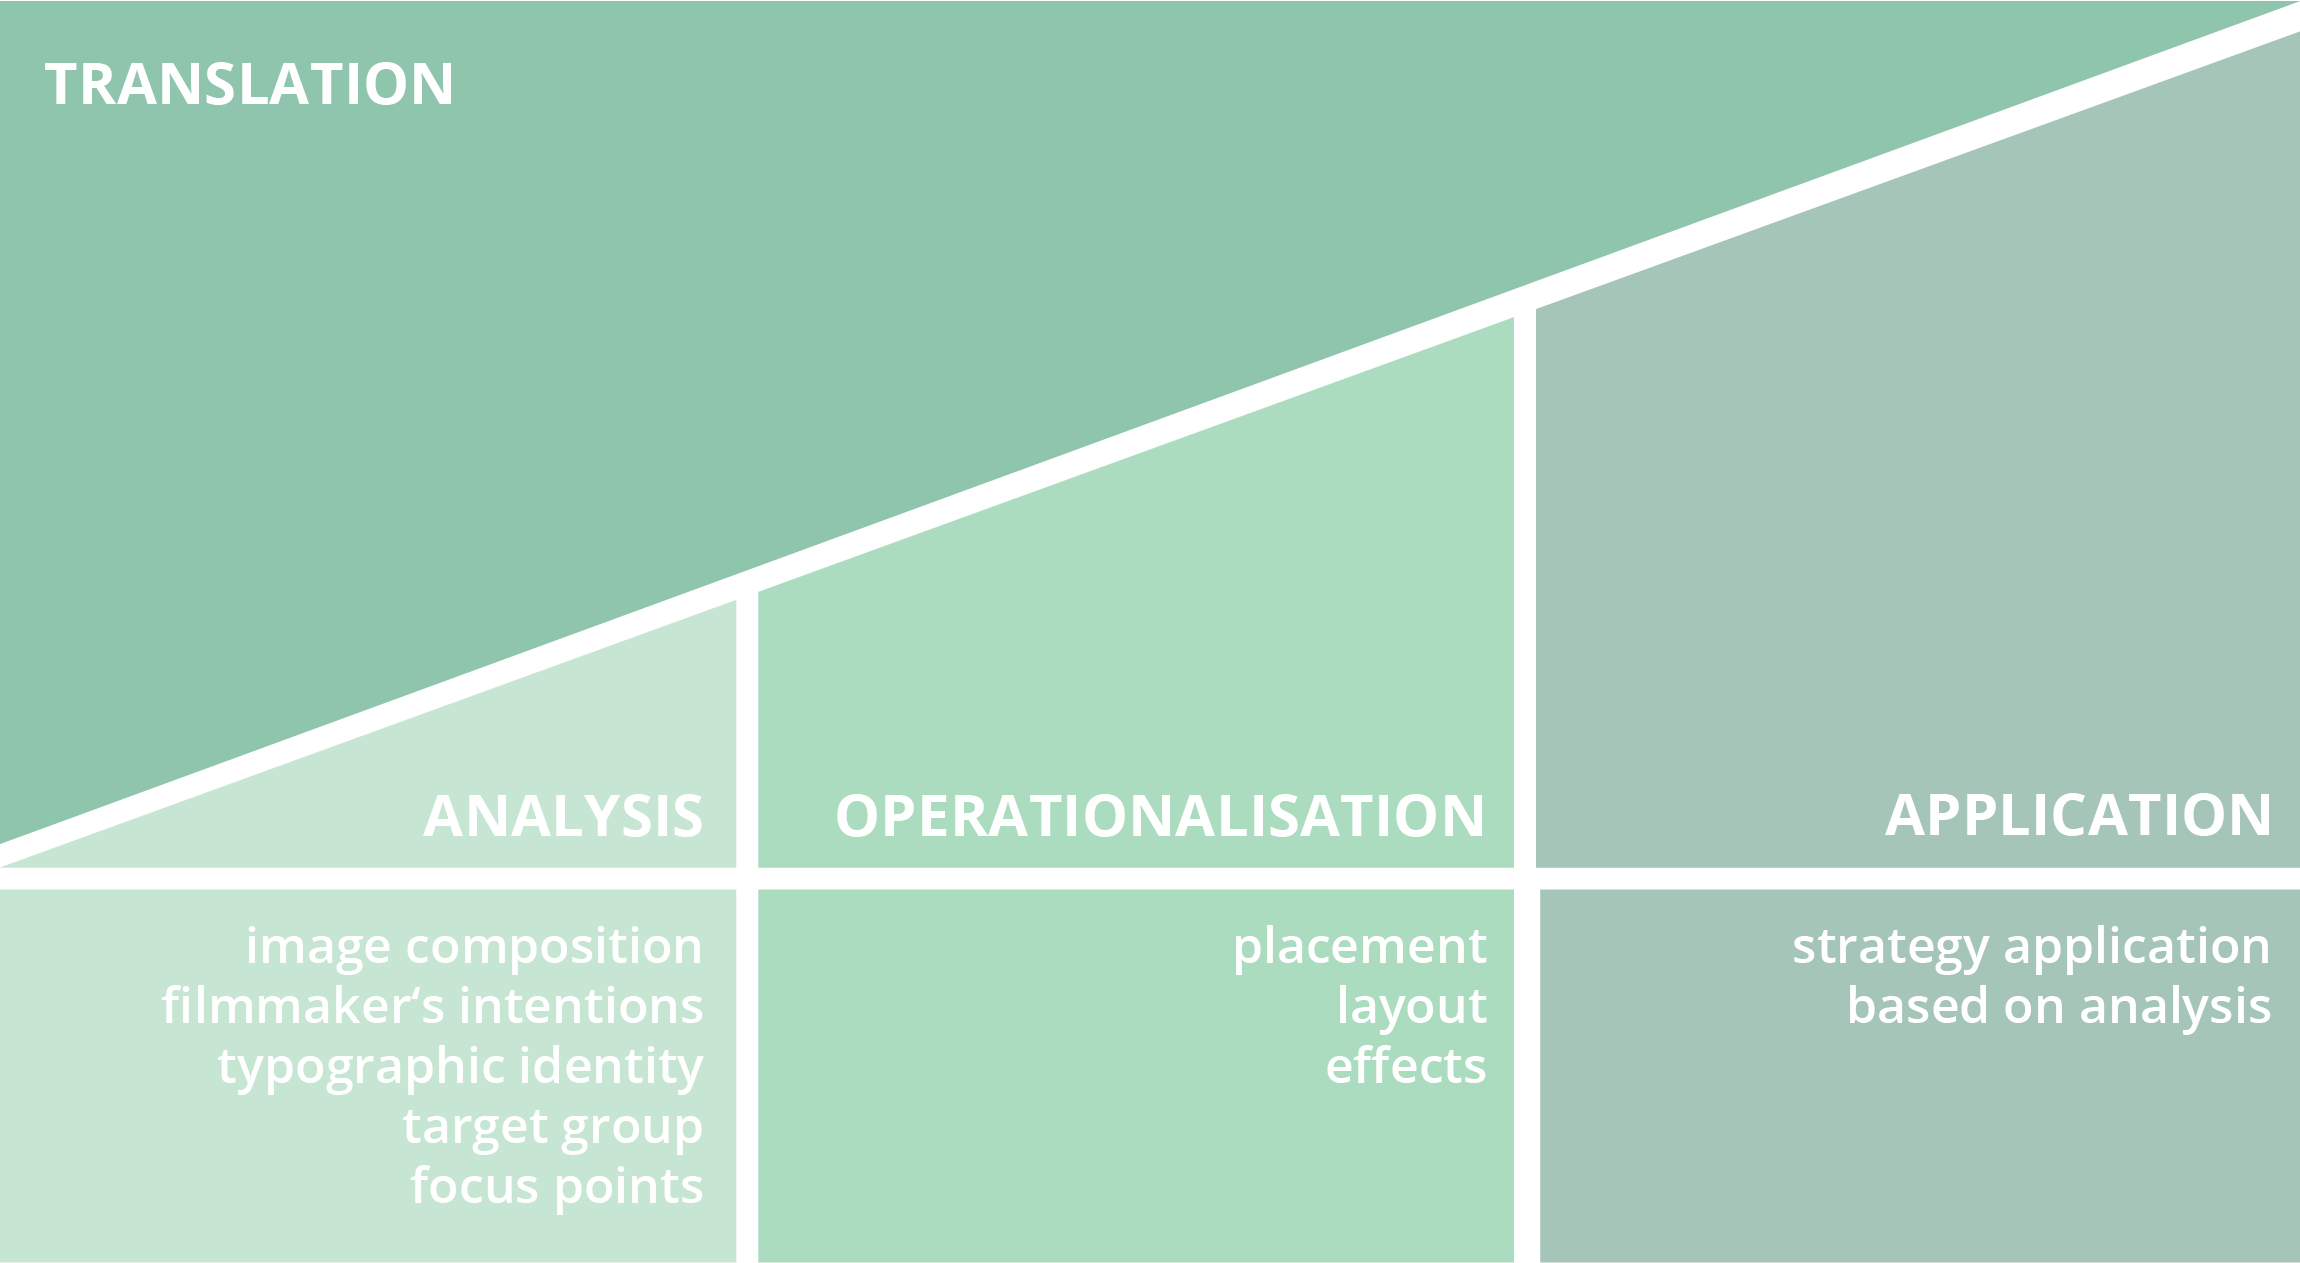
\includegraphics[width=\textwidth]{figures/FIG44chart2.png}
\caption{Detailed proposed workflow for the creation of integrated titles}
\label{fig:FIG44}
\end{figure}

As concepts like these should definitely be tested outside the study they were created for as well as criticised and improved again and again, there is a wide range of possible follow-up studies. The strategies and workflow have so far been tested in the course of a Bachelor thesis, a research project, and in a real-life setting. Especially the Bachelor thesis by \citet{Hevesi2015} led to adjustments based on the student’s feedback. Hevesi created integrated titles for the English short film \textit{Carry On Only} (USA 2013) and did a small eye tracking- and questionnaire-based study with three English native participants and eight German participants dependent on subtitles. Based on the presented \isi{placement} strategies, the workflow, and results from the pilot study in 2012, as well as the eye movements of the English participants, the integrated titles for \textit{Carry On Only} were developed. They followed the film’s \isi{typographic identity} and made use of a few effects (spatial, \isi{typographic}, and display effects). The \isi{eye tracking} data revealed that during the \isi{title display}, the participants spent more time on the image than on titles, they did not show any unnatural searching behaviour and the recorded eye movements did not show signs of stress. In the questionnaire, at least 75\,\% of the participants rated \isi{legibility}, stress, time for \isi{image exploration}, \isi{detail perception}, and effects positively. However, most participants did not really notice the effects or cared much about them. Concerning the workflow, the need for adjustments and changes to the translation during the process was added.

For a further study on the reception of integrated titles by Kruger et al. (\citeyear{Kruger????b}), integrated titles were created for the first 30~minutes of the English blockbuster film \textit{Sherlock Holmes – A Game of Shadows} (USA 2011). As this is quite an action-packed film, it was decided to keep to the conventional position in the bottom-center area of the frame as long as there was no superior position. The titles indicate speaker and \isi{speaking direction}, were placed close to \isi{main focus} points, and made use of spatial and display effects (see \figref{fig:FIG45}, \citealt{Kruger????b}). No need for adjustments of the workflow was observed.

\begin{figure}
\includegraphics[width=\textwidth]{figures/FIG45fig43.jpg}
\caption{Edited scene including integrated titles for \textit{Sherlock Holmes – Game of Shadows} (00:05:38, 00:17:17)}
\label{fig:FIG45}
\end{figure}

\newpage 
The most recent project that made use of the proposed \isi{placement} strategies and workflow took place in cooperation with the filmmaking and production team of \textit{Notes on Blindness} (UK 2016) and was supervised by Pablo Romero-Fresco, who advised concerning \isi{placement} and accessibility. Feedback came from the filmmakers, producers, subtitle professionals (who created the SDH), and Pablo Romero-Fresco. As these integrated titles are targeted at a hearing-impaired audience, \isi{noise indication} and \isi{colour-based speaker identification} were added (see \figref{fig:FIG46}).

\begin{figure}
\includegraphics[width=\textwidth]{figures/FIG46fig44.png}
\caption{Colour-based speaker identification in \textit{Notes on Blindness} (00:03:17)}
\label{fig:FIG46}
\end{figure}

The colours were chosen per speaker and taken from the colours that are present during scenes with that person. Another new feature was the additional indication of speaking volume and source (see \figref{fig:FIG47}).

\begin{figure}
\includegraphics[width=\textwidth]{figures/FIG47fig45.jpg}
\caption{Volume and source indication in \textit{Notes on Blindness} (00:02:53, 00:24:29)}
\label{fig:FIG47}
\end{figure}

\section{Summary}\label{sec:5.4}

Based on the theoretical framework developed in the previous chapters, a basic workflow for the creation of integrated titles was drafted, being the first of its kind. Including the four steps of translation, analysis, operationalisation, and application, it gives an overview over the process behind integrated titles. The analysis should include a discussion of the \isi{image composition} of the film and the filmmaker’s intentions – ideally interview-based – as well as an analysis of the pre-existing text elements and the \isi{typographic identity} they create. Before any decisions concerning the overall concept are made, the target group should be defined and basic focus points be identified. This should result in a concept consisting of the chosen strategies for \isi{placement}, \isi{layout}, and effects which are then applied in the final step. A professional tool that allows this kind of \isi{placement} is \textit{Adobe Premiere Pro}, which is presented in \sectref{sec:7.2.2}. First application tests after the pilot study in 2012 (see \sectref{sec:7.3}) such as the Bachelor’s thesis by \citet{Hevesi2015} provided feedback on the workflow and led to some adjustments that were finally applied in the first real-life and commercial project \textit{Notes on Blindness}, which also highlighted applicability in the area of accessibility.

\largerpage
In order to analyse the reception of both conventional subtitles and integrated titles, \isi{eye tracking} can give insight concerning reaction times, reading durations, and general eye movements across the image. As \isi{eye tracking} was chosen to be the main tool of analysis of the present study, the following chapter gives a basic introduction to \isi{eye tracking} and relevant \isi{eye tracking} areas and studies.